\section{Design of \sys}
\label{s:impl}


In this section, we describe design details of \sys, a
coverage-directed concurrency fuzzer to effectively find concurrency
bugs.
%
The key improvement of \sys lies in adopting interleaving segment
coverage and the coverage-directed interleaving mutation algorithgm
described in \autoref{s:design}.
%
To this end, \sys implements three components, the userspace fuzzer,
target kernel instrumentation, and the execution engine.
%
In the following of subsections, we describe design details and
implementation of each components.


\subsection{Userspace Fuzzer}
\label{ss:fuzzer}



\begin{figure}
  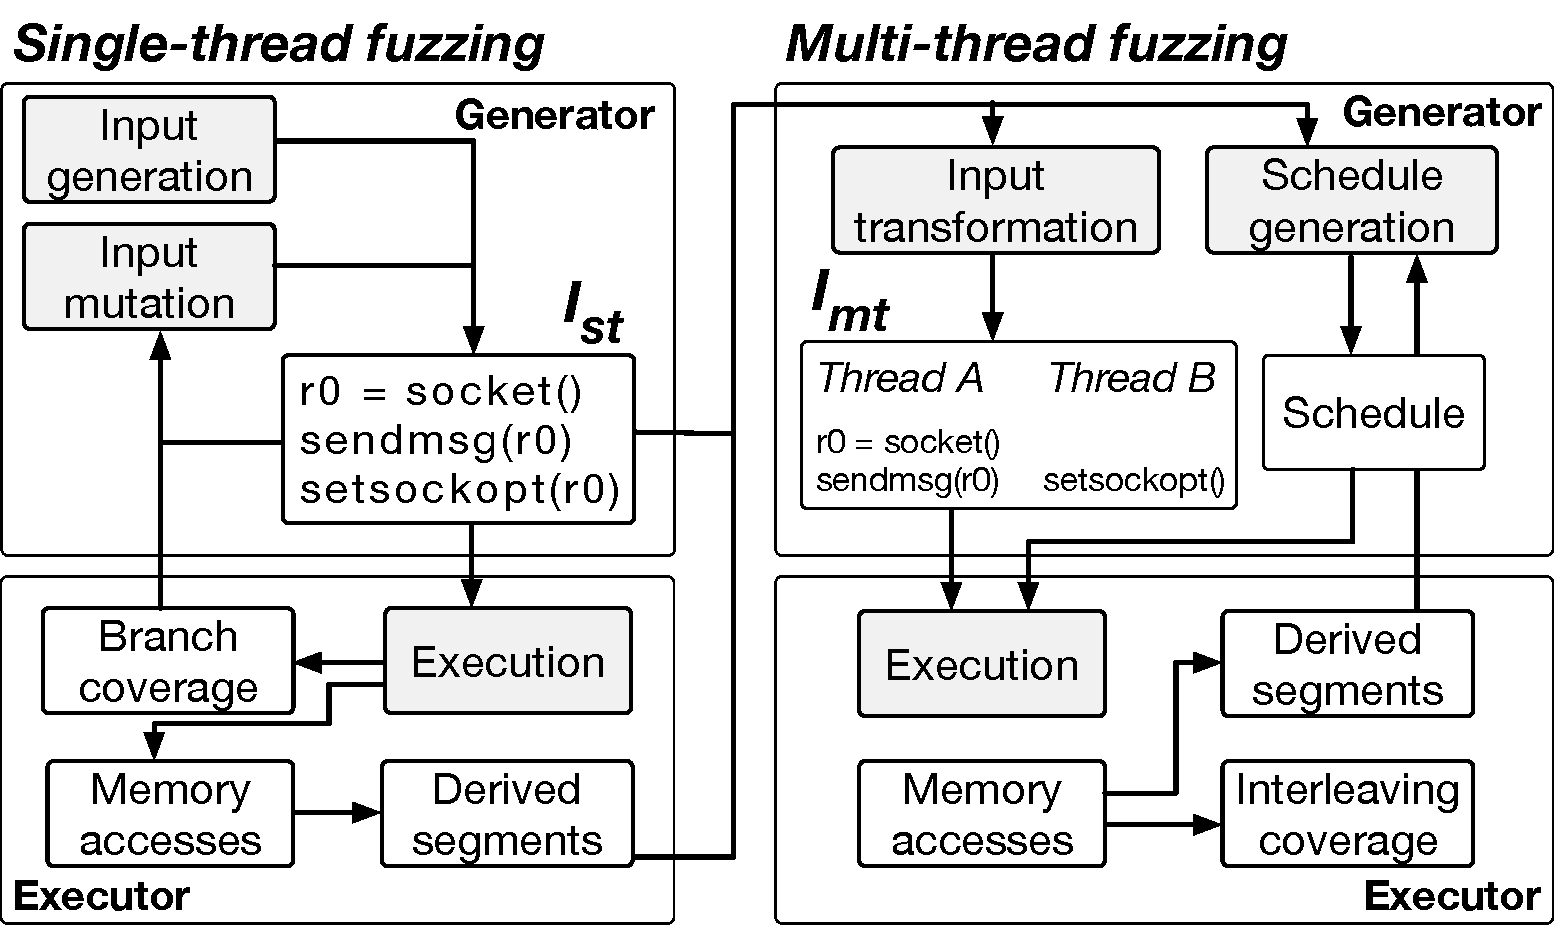
\includegraphics[width=0.9\linewidth]{fig/architecture.pdf}
  \caption{Workflow of \sys \dr{TODO: redraw to describe the workflow}}
  \label{fig:workflow}
\end{figure}


The \sys's userspace fuzzer conducts two-stage pipelined fuzzing.
%
The first stage is single-thread fuzzing which generates a
\textit{single-thread} input program, \ie, a sequence of system calls.
%
While the first stage fuzzing generates and runs sequential inputs to
expand brach coverage, it also finds sequential inputs that include
system calls, called XXX, that may expose new biconflict coverage when
executed concurrently.

\autoref{fig:workflow} describes the workflow of the \sys's userspace
fuzzer.
%


%
The second stage is to explore the interleaving. Given a sequential
input program from the first stage, it constructs a
\textit{multi-thread} input program that executes the XXX syscalls
concurrently.
%
During the second stage fuzzing, the fuzzer keeps generating
interleavings of the XXX syscalls and tracks biconflict coverage for
the concurrent dimension.




A userspace fuzzer implmenets the interleaving mutation algorithm
described in \autoref{s:design}.
%
We choose to implement \sys based on Syzkaller~\cite{syzkaller} which
is a grammar-based grey-box fuzzer since Syzkaller has been found many
bugs for a few years.
%

\PP{Sequential fuzzing}
%
\sys's sequential fuzzing is similar with Syzkaller.

In the first phase fuzzing, \sys make use of branch coverage for the
sequential dimension


KCOV~\cite{kcov}

\PP{Concurrent fuzzing}

%
In order to use interleaving graph as interleaving coverage, we need a
method to store them, and compare them to a new interleaving graph.
%
We choose to use a hash value of

the FNV-1~\cite{fnv, fnv-go}, non-cryptographic hash function,

\PP{Schedule}

A schedule is an outcome of the interleaving mutation.

A schedule contains an initial thread, and a set of scheduling points
indicating an instruction on which preemption occurs.


\subsection{Target Kernel Instrumentation}
\label{ss:instrumentation}

\sys requires to instrument callbacks before all memory access
instructions for tracking memory access operations.
%
% Unlike data race detectors such as KCSAN~\cite{kcsan}, the \sys's
% scheduling mechanism needs to recognize both plane memory accesses and
% annotated memory accesses such as atomic operations.
% %
% We deal with these two types of accesses differently since annotated
% accesses usually are implemented in assembly code, which is hard for a
% LLVM pass to understand.
% %
% In order to instrument plane accesses, we implement a LLVM pass that
% insert callback function calls after memory accesses on LLVM IR.
% %
% Our pass runs after most of binary transfomration is done, so it
% \XXX{...}.
% %
% For annotated instructions, we rely on the functionality of
% KASAN~\cite{kasan} to instrument atomic operations.
% %
% KASAN provides wrapper functions of annotation APIs to call callback
% functions before annotated memory operations, and we instruct the
% wrapper functions to call our callbacks as well.
% %
% Our callbcak functions write memory access operations along with
% various information into a region mmap-ed shared region shared by a
% userspace program (\ie, fuzzer) and a kernel. The information about
% memory operations includes the instruction address, the start address
% of a memory location, and the size of memory access.
% %
% Accordingly, a fuzzer is able to identify what memory access
% operations took place during the execution.

% \sys also requires an additional module called a trampoline that is
% used to suspend and resume a running thread. Details about the
% trampoline are described in \autoref{ss:engine}.


\subsection{Execution Engine}
\label{ss:engine}

\begin{figure}
  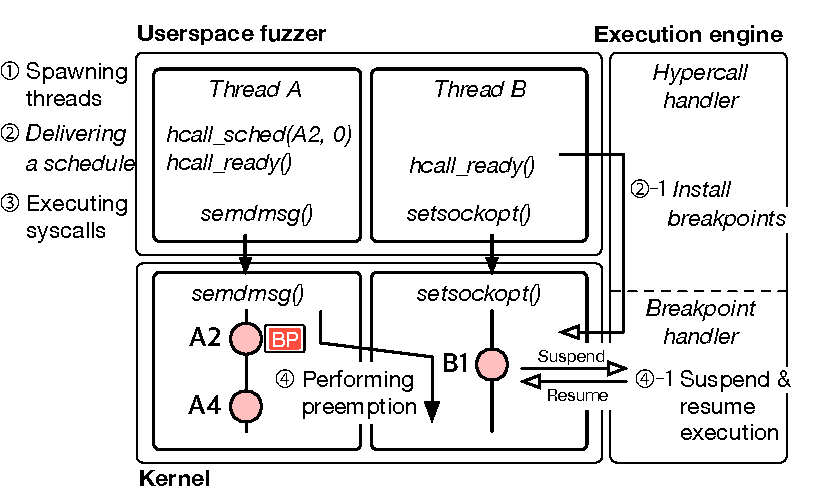
\includegraphics[width=0.9\linewidth]{fig/workflow-hypervisor.pdf}
  \caption{The workflow of the execution engine. \red{IMPORTANT: this
      is copied from AITIA. Need to redraw}}
  \label{fig:workflow-hypervisor}
\end{figure}

We introduce an execution engine in order to enforce an interelaving
provided by a fuzzer.
%
Specifically, the execution engine is to enforce an interleaving of
threads controlled by a fuzzer while all other kernel threads work
ordinarily.
%
During the execution, our hypervisor allows only one thread to execute
to make the execution serialized.
%
We implment the execution engine in the hypervisor layer to make it as
non-intrusive as possible.

\PP{Enforcing interleavings}
%
\autoref{fig:workflow-hypervisor} shows the overall workflow of our
execution engine.
%
The execution engine and a fuzzer communicates through hypercall
interfaces.
%
Scheduling points are sent from a fuzzer to the hypervisor before a
fuzzer executes concurrent syscalls.
%
\dr{TODO: how to send a schedule. what is a form of scheduling points}
A schedule is a specification of ...
%
After the fuzzer sends a schedule, the fuzzer notifies a hypervisor,
and the hypervisor starts executing with the intial thread specified
in the given schedule while other threads are suspended.
%
When the running thread reaches a scheduling point, a hypervisor
performs preemption by suspending the running thread and resuming the
next thread to run in order to enforce the execution order between
memory access operations.
%
\dr{TODO:}
Details about suspending and resuming a thread is described later.
%
\dr{TODO: how to handle missing breakpoints}


\PP{Suspending a thread}
%
A few prior approaches~\cite{ski, snowboard, razzer} suspend a vCPU
instead of a guest thread. While suspending a vCPU grants the ability
to control an interleaving, it is not suitable for our purpose because
suspending a vCPU may unexpectedly suspend another vCPU. An example we
observed is TLB shootdown~\cite{tlbshootdown}. When a vCPU wants TLB
shootdown, it sends inter-process interrupts (IPIs) to all cores and
wait until all cores to execute the TLB shootdown handler.  In this
case, if one vCPU is entirely suspended, the TLB shootdown cannot be
successfully conducted causing the vCPU invoking TLB shootdown
blocked.
%
Therefore, instead of adopting the prior approach, our hypervisor is
designed to suspends and resumes a guest thread.
%
In order to suspend a thread at an arbirary location, we use a
hardware breakpoint functionality~\cite{hwbp} shipped in modern Intel
CPU chipsets.
%
When a guest thread hits a breakpoint, our hypervisor saves its
register values and then changes the program counter of the thread to
an infinite loop called trampoline. In the trampoline, the thread
keeps calling \texttt{cond_resched()} to yield a CPU to make all other
kernel functionalities (\eg, handling the TLB shootdown handler) work
normally. When the guest thread resumes, our hypervisor restores
registers with the values saved when the thread is suspended, and the
thread continues its execution.


\PP{Virtual Machine Instrospection}
%
\dr{Not important contents but too long}
%
In the middle of execution, our hypervisor introspects the target
kernel for two reasons.
%
First, when a breakpoint is hit, it needs to determine whether the
breakpoint is hit by a fuzzer-controlled thread.
%
As a hardware breakpoint does not distinguish the running context of a
kernel, if the context switch happens, a breakpoint may be hit by
another thread or an interrupt handler, making the execution out of
expectation.
%
The hypervisor recognizes a running context using \texttt{task_struct}
which holds the thread description, and the per-cpu
\texttt{preempt_count} variable indicating what context the thread is
in (\eg, a task context for running a syscall, or a hardIRQ context to
handle hardware interrupts).
%
If a breakpoint is hit by a context other than the fuzzer-controlled
thread, our hypervisor ignores it and keeps the breakpoint.

Second, when a running thread tries to acquire a lock, our hypervisor
inspects the lock is held by a suspended thread.
%
When the suspended thread already acquires a lock while the running
thread wants to hold the same lock, the whole execution cannot make a
progress, because our hypervisor forces the lock-holding thread to
suspend.
%
Therefore, our hypervisor inspects whether the running thread is going
to be blocked due to the lock contention, and if it is, our hypervisor
takes control from the running thread to the suspended thread.
%
Inspecting the lock contention is conducted by hooking lockdep
functions~\cite{lockdep} that are commonly called from synchronization
prmitives.
%
When the lockdep functions are called, our hypervisor determins
whether the running thread can make a progress through various
information such as the address of the synchronization primitive, and
operation type (\ie, lock, unlock, and trylock).


\subsection{Implementation}
\label{ss:impl}

We implement \sys in various software layers.
%

%
To allow 


We use scc~\cite{scc} and sloccount~\cite{sloccount} to measure LoC of
GO and C respectively.


%%% Local Variables:
%%% mode: latex
%%% TeX-master: "p"
%%% End:
